


\section{Experiment Results\label{sec:results}}

%when the available clues for alignment are sparse, we have performed comparative evaluation of our model against several baselines.

\begin{table}
	\centering
	% \small
	\scriptsize
	\begin{tabular}{lrrrr}
		\toprule
		\multirow{2}{*}{$\bf DBP15K_{FR-EN}$} & \multicolumn{2}{c|}{$\bf FR \rightarrow EN$} & \multicolumn{2}{c}{$\bf EN \rightarrow FR$} \\
		& \bf Hits@1 & \bf Hits@10 & \bf Hits@1 & \bf Hits@10 \\
		\midrule
		\rowcolor{Gray}JE & 15.38 & 38.84 & 14.61 & 37.25 \\
		MTransE & 24.41 & 55.55 & 21.26 & 50.60 \\
		\rowcolor{Gray}JAPE (SE) & 29.63 & 64.55 & 26.55 & 60.30 \\
		JAPE (SE+AE) & 32.39 & \bf 66.68 & 32.97 & \bf 65.91 \\
		\rowcolor{Gray} \bf \HRGCN (SE) & 33.43& 35.72& 31.22& 34.65 \\
		\bf \HRGCN (S$\oplus$A) & 23.8 & 32.4 & 20.4 & 27.5 \\
        \rowcolor{Gray} 	\bf \HRGCN (SE+AE) & \bf 44.82 & 56.68 &\bf 41.08 & 52.95 \\
		\bottomrule
	\end{tabular}
	\caption{Performance on $DBP15K_{FR-EN}$ dataset.}
	\label{cross}
\end{table}

\begin{table}
	\centering
	% \small
	\scriptsize
	\begin{tabular}{lrrrr}
		\toprule
		\multirow{2}{*}{\bf Models} &  \multicolumn{2}{c|}{$\bf Baidu \rightarrow Wiki$} & \multicolumn{2}{c}{$\bf Wiki \rightarrow Baidu$} \\
		& \bf Hits@1 & \bf Hits@10 & \bf Hits@1 & \bf Hits@10 \\
		\midrule
		\rowcolor{Gray} JE & 14.8 & 21.6 & 13.2 & 20.3 \\
		ITransE$'$ & 19.4 & 25.5 & 17.6 & 24.8 \\
		\rowcolor{Gray} \GCN & 17.1 & 27.3 & 15.7 & 25.9 \\
		\HGCN & 19.5 & 29.6 & 19.4 & 29.5  \\
		\rowcolor{Gray} \RGCN & 37.3 & 51.5 & 34.8 & 51.6 \\
		\bf \HRGCN (w/o $X$) & 15.0 & 21.7 & 14.5 & 21.5 \\
		\rowcolor{Gray} \bf \HRGCN (SE+AE) & 58.3 & 67.1 & 57.8{\tiny } & 65.7 \\
		\bf \HRGCN (S$\oplus$A) & \bf 65.1 & \bf 71.7 & \bf 62.2 & \bf 71.4\\
		\bottomrule
	\end{tabular}
	\caption{Performance on WBD dataset.}
	\label{f1}
\end{table}
\subsection{Overall Performance\label{overall}}
We evaluate our approach on four variant implementations: (1) a two-layered \HRGCN (S$\oplus$A) ($\oplus$ represents concatenation) which directly uses concatenated vectors
introduced in Section~\ref{sec:combine} as input node features, (2) a two-layered \HRGCN (SE+AE) which combines semantic embedding and
attribute embedding, (3) a two-layered \HRGCN (SE) which only performs semantic embedding with pre-trained word vectors, (4) two-layered
\HRGCN (w/o X) which does not use the predefined feature vectors mentioned in Section~\ref{subsection:Node
		Representations} as the input.

\cparagraph{Results on $\bf DBP15K_{FR-EN}$} Table~\ref{cross} reports the results of all the compared approaches on $DBP15K_{FR-EN}$
dataset. We apply each approach
 to two alignment directions: French to English and vice versa. This dataset requires us to handle
cross-lingual data through rough machine translation which is likely to introduce lots of noise. We report the performance of JAPE on the
two implementations presented at
 ~\cite{sun2017cross} when using structure embedding (SE), and structure and attribute joint embedding (SE+AE).
For Hits@1, our \HRGCN (SE+AE) outperforms all other approaches by delivering the highest score. This is due to the capability of \HRGCN
(SE+AE) in preventing noisy nodes from driving the \KG representations. For Hits@10, JAPE (SE+AE) gives the best performance, which
translates to a improvement of 10\%$\sim$13\% over \HRGCN (SE+AE). However, our approach has the advantage for not relying on aligned
relations and attributes and thus has lower overhead.


\cparagraph{Results on WBD} Table~\ref{f1} reports the performance of all models on WBD dataset. While the vanilla \GCN performs worse than
exhibiting alignment models, by adding highway gates to control the noise, \HGCN is able to outperform all existing approaches. By
incorporating node representation and \RGCN, our \HRGCN (S$\oplus$A) model delivers the best Hits@k score in both alignment directions,
improving upon the best-existing method -- ITransE$'$ by 45.7\% and 46.2\% for Hits@1 and Hits@10 respectively in the direction of
Baidu$\rightarrow$Wiki. This shows that our model has a distinct advantage in entity alignment task over existing approaches.

In addition, we find that the performance of \HRGCN (SE+AE) and \HRGCN (S$\oplus$A) is very different on the two datasets. We provide a further discussion on the two strategies for exploiting the semantic and attribute embeddings in Section~\ref{sec:analysis}.


\subsection{Analysis\label{sec:analysis}}


%An extra advantage of GCN is that we can stack multiple convolution layers to capture more global and larger contextual and neighboring characteristics

We now provide a detailed analysis to compare different approaches.

\cparagraph{\GCN vs. prior methods}
From Table~\ref{f1}, \GCN-based model outperforms JE regarding all the Hits@k and performs better than ITransE$'$ in Hits@10 for both alignment directions. As aforementioned, \GCNs leverage convolutional layers to characterize an entity through careful investigations about its neighbors, including both neighboring entities and attribute values, which can provide more fine-grained and accurate modeling and representation for the target entity.

\cparagraph{\GCN vs. \RGCN} As shown in Table~\ref{f1}, comparing with \GCN, the \RGCN-based model further boosts the performance by 20.2\% and 24.2\% for Hits@1 and Hits@10 in the direction of Baidu$\rightarrow$Wiki. And in the opposite alignment direction, \RGCN also has obvious advantage. This verifies the fact that introducing highly multi-relational information to \GCN framework can achieve significant improvements on KG embedding.

\cparagraph{(SE+AE) vs. (S$\oplus$A)}
According to the results listed in Table~\ref{f1}, \HRGCN (S$\oplus$A) outperforms \HRGCN (SE+AE) for Hits@1 and Hits@10 in both alignment directions. However, \HRGCN (SE+AE) achieve better performance than \HRGCN (S$\oplus$A) on $DBP15K_{FR-EN}$ dataset. This might be because the data of the two \KGs in $DBP15K_{FR-EN}$ dataset are all from DBpedia, their normalized attribute vectors could be very similar, even exactly match in some dimensions. But the data in WBD dataset was extracted from two heterogeneous KGs, their attribute vectors may be very different. When two attribute vectors with large differences pass through \HRGCNs, it may amplify their difference. On the contrary, two very similar vectors may be more similar after encoded by \HRGCNs.


\cparagraph{(SE+AE) vs. (SE)}
Comparing the results of \HRGCN (SE+AE) and \HRGCN (SE) in Table~\ref{cross}, we can see that adding attribute embedding greatly improves the performance, resulting in a 11.39\% jump in Hits@1 and a 20.96\% jump in Hits@10 in the direction of FR$\rightarrow$EN. It shows that the attribute information is very useful for entity alignment.
From Table~\ref{f1}, when comparing our full model \HRGCN with \HRGCN (w/o $X$), we find that removing the predefined input feature matrix $X$ leads to a drop of 43.3\% for Hits@1 and 45.4\% for Hits@10. This confirms that initializing entity representations using pre-trained word embeddings and normalized attribute vectors is very helpful in aligning entities from different KGs.

\cparagraph{Performance comparing under sparse alignment clues}
To further show the effectiveness of our model under sparse alignment clues, we divide the WBD test set into four subsets according to the difference between the number of neighbors of each entity pair, and compare the performance (in Hits@1) of ITransE$'$, \GCN and \HRGCN (combined semantic embedding and attribute embedding) on the four subsets.
%Figure~\ref{subset} shows the $\mathrm{F}_1$ scores of on the five subsets.

As shown in Figure~\ref{subset}, we can see that when the number of neighbors differs by no more than 2, the Hits@1 scores of all three models are over 20\%.
But when the difference between the entity pairs' neighborhoods becomes more prominent,
our \HRGCN model tends to deliver more clear improvement. We can also see that our \HRGCN wins \GCN in every subset.
This is mainly because introducing highly multi-relational information to \GCN with highway gates can help our model better embed the relational structure information and focus on the most discriminative aspects from the target entity's neighbors, thus lead to more accurate representations.
%, the three models all perform well and the scores are not far-off. However, when the difference in the number of neighbors gradually increases, the gap between JE and the other two models also grows.
\begin{figure}
	\centering
	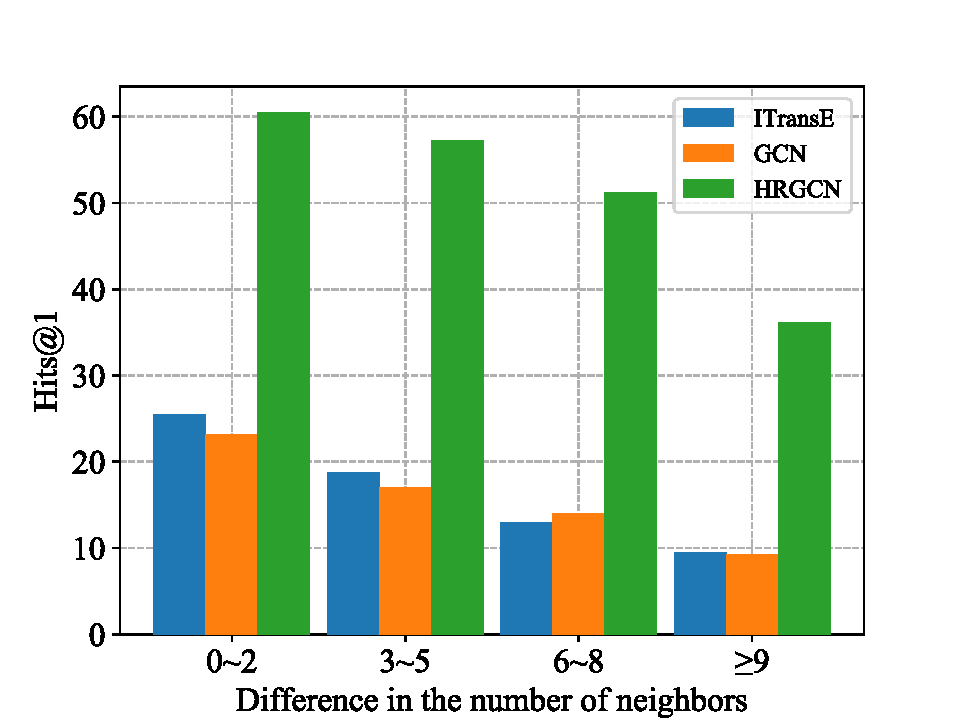
\includegraphics[width=0.8\linewidth]{figures/graph4.pdf}
	\caption{Hits@1 of ITransE$'$, \GCN and \HRGCN on the four WBD subsets. 0$\sim$2 denotes the subset in which the number of neighbors differs from 0 to 2 for each entity pair, and similar for the remaining subsets.}
	\label{subset}
\end{figure}

Moreover, from WBD test set, we randomly choose some examples that our \HRGCN model can correctly align but ITransE$'$ fails in Table~\ref{example}, as well as their neighbor information, i.e., number of neighbors, number of values, number of potentially overlapped neighbors or values for each pair.
We can find that although several entities have dozens of neighbors in their corresponding KGs, but their similar or overlapped neighbors are quite few, showing again that
%the number of similar neighbors of these entity pairs is no more than 6 which is very small compared to the number of their neighbors. This indicates that
the available clues for entity alignment are sparse and ITransE$'$ may not perform well in this circumstance, while our \HRGCN model can still identify useful structure information from those limited clues.

We can also observe from Table~\ref{example} that values play an important role in entity alignment.
For instance, in the entity pair about \textit{Hubei Province}, nearly half of the neighbors for each entity are values, and among all 5 similar neighbors, 3 of them are actually values,
which provide crucial supporting evidence for the final prediction. Unfortunately, ITransE$'$ does not utilize those information, thus is unable to collect sufficient evidence.

\begin{table}
	\centering
	\scriptsize
	\begin{tabular}{ccccc}
		\toprule
		\multirow{2}{*}{\bf Aligned Entities} & \bf \#Neighbors & \bf \#Similar & \bf \#Values & \bf \#Similar \\
		&\bf  Wiki \& Baidu &\bf  Neighbors &\bf  Wiki \& Baidu &\bf  Values \\
		\midrule
		Deng Jiaxian & 10 \& 33 & 5 & \ 3 \& 11 & 2\\
		Hubei Province & 21 \& 50 & 5 & 10 \& 19 & 3\\
		European Union & 66 \& 35 & 6 & 18 \& 8\ \ \ & 2\\
		%Huazhong University of & \multirow{2}{*}{11 \& 32} & \multirow{2}{*}{4} & \multirow{2}{*}{8 \& 6} & \multirow{2}{*}{1}\\
		%Science and Technology & & & & \\
		%Huazhong University of Science and Technology & 11 \& 32 & 4 & 8 \& 6 & 1 \\
		Confucius & 10 \& 20 & 4 & 7 \& 3 & 2\\
		\bottomrule
	\end{tabular}
	\caption{The statistics of example entity pairs, which our HRGCN model correctly aligns but ITransE$'$ fails.}
	\label{example}
\end{table}


\cparagraph{Highway gates}
Adding more \HRGCN layers can help the center entities obtain information from neighbors that are multiple hops away. However, it might also introduce noisy information from the exponentially increasing neighbors, leading to significant decline in performance as shown in Figure~\ref{highway} when no highway gates are used. We can observe that the performance of two-layered \RGCNs with highway gates improves upon one-layered \RGCN. Then by adding more layers the performance of highway \RGCNs decreased slowly, but much slower than \RGCNs without gates. This confirms that the highway gates effectively control the required balance of neighbor information transmission in \RGCNs.

In addition, from Table~\ref{f1}, we can observe that the \GCN or \RGCN-based models with highway gates consistently achieve better performance than no-highway ones. This indicates that highway gates can effectively improve the performance of both multi-layered \GCN and \RGCN models.
\begin{figure}
	\centering
	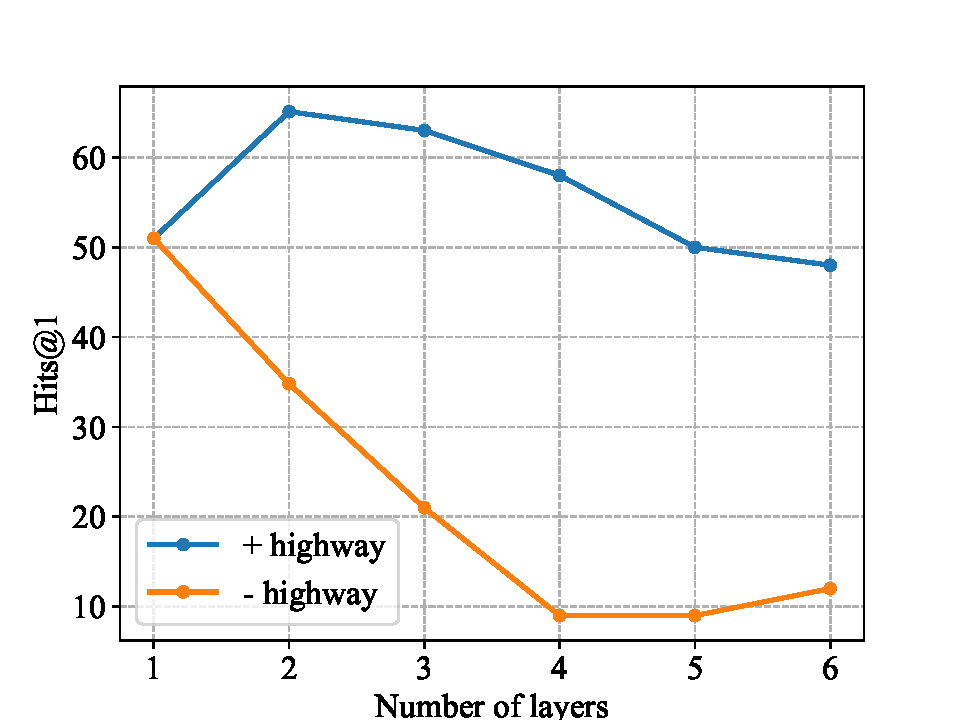
\includegraphics[width=0.8\linewidth]{figures/graph3.pdf}
	\caption{The effect of adding more \RGCN layers in terms of Hits@1 over the test set of WBD with and without the highway gates.}
	\label{highway}
\end{figure}
